\documentclass[letterpaper,12pt]{report}

%%%% IMPORTANT %%%%
% Set page's format followed the guideline
\usepackage[left=1.5in,right=1in,top=1in,bottom=1.25in,head=0.5in]{geometry}
% This is to use with \doublespacing for text in the dissertation
\usepackage{setspace}
%%%% END IMPORTANT %%%%
%%%% OTHER USEFUL PACKAGES %%%%
\usepackage{amsmath}
\usepackage{amssymb}
\usepackage{amsfonts}
\usepackage{latexsym}
\usepackage{lipsum}
\usepackage{multicol}
\usepackage{accents}
\usepackage{harpoon}
\usepackage{wrapfig}
\usepackage{float}
\usepackage{tabularx}
\usepackage{euscript}
\usepackage{color}
\usepackage{xcolor}
\usepackage{graphicx}
\usepackage{float}
\usepackage[caption = false]{subfig}	
\usepackage{epsfig}
\usepackage{hyperref}

\usepackage{fancyhdr}

\usepackage{textcomp}
\usepackage{cite}
\usepackage{pdfpages}
\usepackage{xparse,mathtools}

\usepackage{algorithm}
\usepackage{algpseudocode}
\usepackage{bibentry}

\usepackage{bibunits}

\DeclareMathAlphabet{\pazocal}{OMS}{zplm}{m}{n}
\newcommand{\Is}{\pazocal{I}}
\newcommand{\Ws}{\pazocal{W}}
\newcommand{\Vs}{\pazocal{V}}
\newcommand{\BigO}{\mathcal{O}}
\newcommand{\Ys}{\pazocal{Y}}
\newcommand{\Xs}{\pazocal{X}}
\newcommand{\Ns}{\pazocal{N}}
\newcommand{\Us}{\pazocal{U}}
\newcommand{\As}{\pazocal{A}}
\newcommand{\Bs}{\pazocal{B}}
\newcommand{\Cs}{\pazocal{C}}
\newcommand{\Ds}{\pazocal{D}}
\newcommand{\Gs}{\pazocal{G}}
\newcommand{\Qs}{\pazocal{Q}}
\newcommand{\Rs}{\pazocal{R}}
\newcommand{\Es}{\pazocal{E}}
\newcommand{\Ts}{\pazocal{T}}
\newcommand{\Ls}{\pazocal{L}}
\newcommand{\Fs}{\pazocal{F}}
\newcommand{\Ss}{\pazocal{S}}
\newcommand{\fs}{\mathbf{f}}
\newcommand{\gs}{\mathbf{g}}
\newcommand{\vs}{\mathbf{\upsilon}}
\newcommand{\Ps}{\pazocal{P}}
\newcommand{\ps}{\mathbf{p}}
\newcommand{\ds}{\mathbf{d}}
\newcommand{\Js}{\pazocal{J}}
\newcommand{\Ms}{\pazocal{M}}
\newcommand{\Ks}{\pazocal{K}}

\newtheorem{definition}{Definition}
\newtheorem{problem}{Problem}

\usepackage[nottoc,notlot,notlof]{tocbibind}
\usepackage{titlesec}

% Define the chapter style: titlesec manual
\titleformat{\chapter}[display]{\normalfont\bfseries\LARGE\filright}
{\LARGE{\chaptertitlename} \thechapter}{1pc}{}

% == Customizations ====================================================
\DeclareRobustCommand{\harpoon}{\accentset{\rightharpoonup}}
\allowdisplaybreaks

% \usepackage{lmodern}
% \usepackage{tgschola}
% == Page Style ========================================================
\pagestyle{fancyplain}
\renewcommand{\headrulewidth}{0.0pt} % gets rid of lines on header
\fancyhead{}						 % clears all header and footer fields
\fancyfoot{}
\fancyhead[R]{\thepage}              % inserts page number in top right

\begin{document}
% \fontfamily{cmss}\selectfont 

% == Use fake numbering until abstract =================================
\pagenumbering{Alph}

% == Title Page +=======================================================
\newpage
\thispagestyle{empty}
\singlespacing

\begin{center}

\null

\vspace{1.5in}

University of Nevada, Reno \\

\vspace{1.5in}

\textbf{Title of Your Dissertation}

\vspace{1.5in}
% Uncomment the below for either Master or PhD
% For dissertation
A dissertation submitted in partial fulfillment of the \\
requirements for the degree of Doctor of Philosophy in\\
Computer Science \& Engineering\\
% For thesis
% A thesis submitted in partial fulfillment of the \\
% requirements for the degree of Master of Science in \\
% Computer Science \& Engineering \\
\vspace{1in}

by

\vspace{0.25in}
John Doe
\vspace{0.5in}

Prof. Dr. Jane Doe - Dissertation Advisor \\
August 2020 \\

\end{center}

% == Copyright =================================================
\newpage
\thispagestyle{empty}
\hbox{\hfil}\vspace{4in}\begin{center}
\textbf{Copyright by John Doe 2020\\
All Rights Reserved}
\end{center}

% == Committee Approval =================================================
% \thispagestyle{empty}
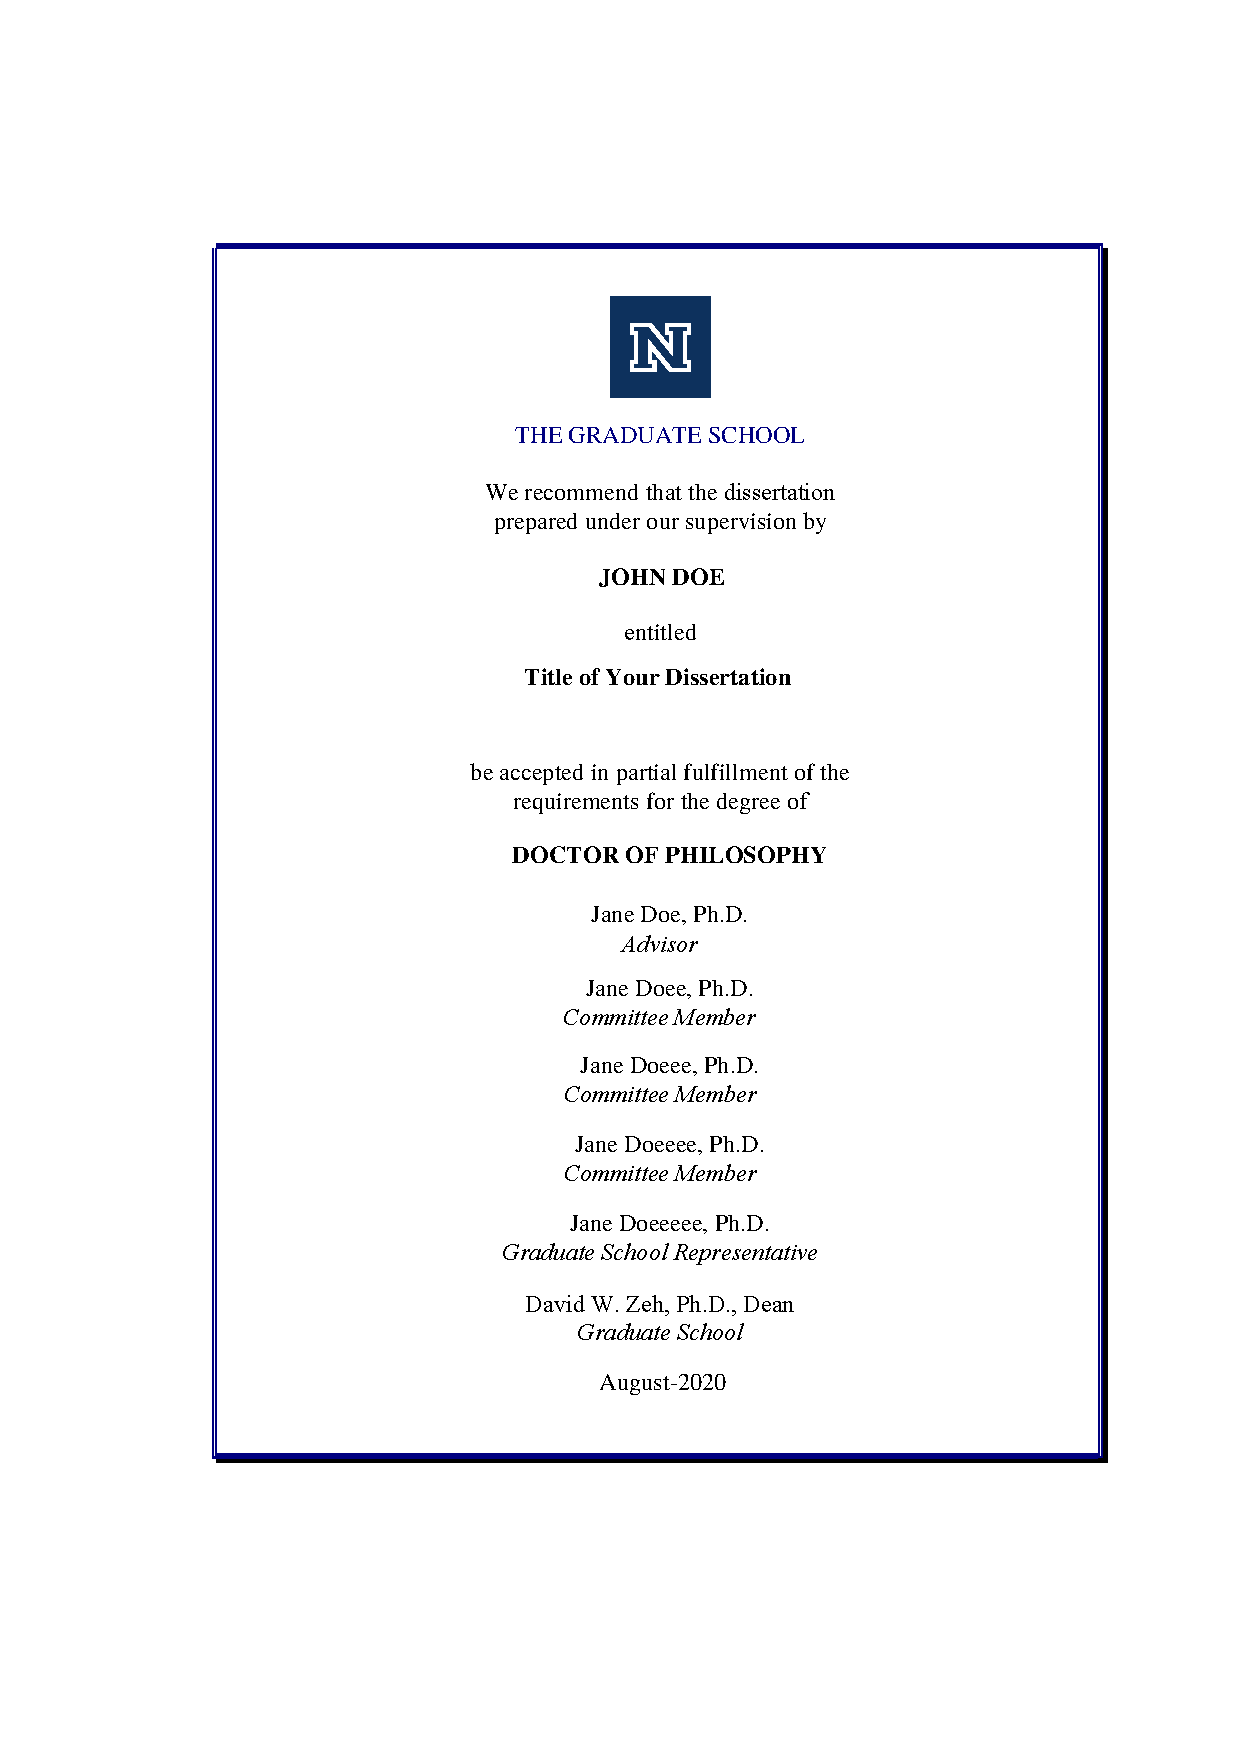
\includepdf[pages={1}]{CommitteeApprovalForm.pdf}

% == Set page numbering style ============================================
\pagenumbering{roman}
\setcounter{page}{0}

% == Abstract ===========================================================


\newpage
\onehalfspace
\begin{abstract}
\thispagestyle{fancyplain}
\doublespacing
\textbf{Please follow the official guidelines at: } \\
\url{https://www.unr.edu/grad/student-resources/filing-guidelines}
\end{abstract}

% == Set page number ====================================================
\setcounter{page}{3}
\doublespacing

% == Dedication ==========================================================
\newpage
\begin{center}
\section*{Dedication}
Dedicated to my parents.
\end{center}

% == Acknowledgments ====================================================
\newpage
% \begin{center}
\section*{Acknowledgments}
Acknowledgements go here
% \end{center}

% == Table of contents ===================================================
\newpage
\renewcommand*\contentsname{Table of Contents}
\tableofcontents

\newpage
\listoftables

\newpage
\listoffigures

% == Set new page number style ===========================================
\newpage

\pagenumbering{arabic}
\setcounter{page}{1}
\linespread{2}

% == Begin thesis content ================================================
\chapter{ Overall Guideline }\label{chap:intro}
\section{Overview}
{\color{red}\textbf{All relevant forms could be found here:~\cite{unr-2020} and ~\cite{unr-2020-forms}}.} \\

Students who have enrolled in dissertation or thesis credits will prepare a manuscript to publish through ProQuest/UMI Dissertation Publishing. You own and retain the copyright to your manuscript. The Graduate School collects the manuscript via electronic submissions only. All manuscripts are made available through ProQuest Dissertations and Theses database (PQDT), in ProQuest/UMI’s Dissertation Abstracts International, and through UNR’s institutional repository, ScholarWorks. \\

Getting started with campus resources:

\begin{itemize}
    \item Office of Human Research Protection
    \item Campus computer Help Desk @One: 775- 682-5000
    \item ProQuest Help Line: 877-408-5027 (8am-5pm Eastern time)
    \item For specific questions call the Graduate School Graduation staff at (775) 784-6869
\end{itemize}

\begin{figure}[h!]
    \centering
    \includegraphics[width=0.5\columnwidth]{PNG/logo.png}
    \caption[Shorter and nicer description]{The Pack. This is an example how to add figure. Shouldn't show this such long caption in the Table of Figures page, use the shortened version in the square brackets instead.}
    \label{fig:my_label}
\end{figure}

\section{Important dates and milestones for graduating students}

\begin{itemize}
    \item Contact your advisor to discuss department considerations and potential dates for your defense.
    \item Contact the Graduate School to ensure your progression paperwork has been approved.
    \item View important dates and purchase a graduation application through MyNevada for your graduation semester.
    \item Doctoral students must submit dissertation title for the commencement program.
    \item Schedule defense date with entire advisory committee in accordance to graduation deadlines.
    \item Submit all forms and final manuscript to the Graduate School by established deadlines.
\end{itemize}

\section{Electronic Manuscript submission}
ProQuest Electronic Submission Site: \href{http://www.etdadmin.com/unr}{http://www.etdadmin.com/unr}\\

Set up an account with ProQuest and wait for a password sent via email. ProQuest offers email and phone support, 1-877-408-5027, frequently asked questions, etc. Visit the site early to familiarize yourself with the submission process.

\section{Checklist to complete electronic submission}
All relevant forms could be found here:~\cite{unr-2020} and ~\cite{unr-2020-forms}.
\begin{itemize}
    \item \textbf{Notice of Completion Form} (bring to the defense for committee signatures) - This form includes all committee signatures AND the Graduate Program Director’s signature.
    \item \textbf{Final Review Approval Form}- This form serves as the final approval from your advisor. The Graduate School will accept the dissertation/thesis after the date listed on the form. The approval date on the form indicates the student’s submission can be accepted.
    \item \textbf{Committee Approval Page} - Use online Word document template (NO SIGNATURES and no page number). This page will be merged into your manuscript to acknowledge committee members.
    \item \textbf{Filing for Copyright Registration} (optional) - Students have the opportunity to register a copyright of the graduate work with the U.S. Copyright Office. It is strictly optional, and there is a \$55.00 fee associated with the service and is paid online with student submission.
    \item \textbf{Processing fee} - \$85 thesis / \$95 dissertation. Due to COVID-19, the process has changed. Log into your Student Center in MyNEVADA. Under the Finances section, click on the link “Purchase Miscellaneous Items.” Select the applicable processing fee to pay (Dissertation or Thesis) and complete the transaction. You will receive a receipt that generates overnight.  Please keep this item as proof of payment for your records. Our office will automatically check for payment posted.
    \item \textbf{Survey of Earned Doctorates} (doctoral students only) - \href{https://sed-ncses.org/login.aspx}{Link}
\end{itemize}

\chapter{ Formatting your dissertation or thesis }\label{chap:related_work}
\section{Margins and spacing}
Example fonts in Latex could be found here\cite{latex-font}.\\

\begin{itemize}
    \item Left margin: 1.5” from left edge of page
    \item Right margin: 1.0” from right edge of page
    \item Top margin: 1.0” from top edge of page
    \item Bottom margin: 1.25” from bottom edge of page 
\end{itemize}

\begin{table}[]
\centering
\caption{Example of a table.}
\label{tab:complexitylocal}
\begin{tabular}{|l|l|}
\hline
\textbf{Year} & \textbf{Name} \\ \hline
\end{tabular}
\end{table}

\section{Fonts}
Fonts should be easy to read. Times New Roman, Arial or a similarly clear font is preferred; type size must be 10, 11, or 12 point. Script and italic typefaces are not acceptable except where absolutely necessary i.e. in Latin designations of species, etc. \\
In preparing your dissertation or thesis for electronic submission, you must embed all fonts. In Microsoft Word 2013, this is done by accessing the FILE menu; select OPTIONS, select SAVE. From the SAVE menu check the box by” Embed fonts in the file”. If the file size is a concern, check the box next to “Do NOT embed common system fonts”. \\
Large tables, charts, etc., may be reduced to conform to page size, but the print must remain clear enough to be readable. You can also attach a PDF for electronic submissions.

\section{Page numbering}
Every page, with the exception of the title page, the copyright page, and the committee approval page is numbered in the upper right hand corner, one half inch from the top of the page and one inch from the right edge of the page. Do not underline or place a period after the number. Do not use a running header. \\
\begin{itemize}
    \item The prefatory materials (abstract, acknowledgements, table of contents, etc.) are numbered in lower case Roman numerals (i, ii, iii, iv…). Insert a section break after the Roman numerals to create different page numbering styles.
    \item The first page of the main text and all subsequent pages are continuously numbered in Arabic numerals beginning with 1 until the final page number (1, 2, 3, 4…).
    \item Do NOT number appendices or pages of additional material with numbers such as 4a or A-1.
\end{itemize}

\section{Tables and appendices}
Tables and appendices are part of the document and must conform to the same margin and page numbering requirements.

\section{Sequence of pages}
Assemble pages in the following order:

\begin{itemize}
    \item Title page *no page number* (create according to example provided)
    \item Copyright Notice *no page number* (optional - see example)
    \item Committee Approval Page *no page number* (use\cite{unr-2020-forms} NO SIGNATURES on this page)
    \item Abstract (begins lower case Roman numerals i, ii, iii…)
    \item Dedication (optional)
    \item Acknowledgments (optional)
    \item Table of Contents
    \item List of Tables
    \item List of Figures
    \item Body of Manuscript (begins Arabic numbering 1, 2, 3…)
    \item Back Matter (appendices, notes, bibliography, etc.)
\end{itemize}

\section{Title page}
\begin{itemize}
    \item Do not number the title page
    \item Center each line of type
    \item Use BOLD text type for the manuscript title
    \item The date listed is the month and year in which you will graduate. The only acceptable months are May, August, and December (graduation cycles).
\end{itemize}

\section{Copyright page}
No page number on this page. Although not required, we strongly recommend you insert a copyright notice in your manuscript following the title page. Essential components of the copyright notice are: copyright symbol, full legal name of author, and year of first publication. Follow the format of the sample provided below.

\section{Committee approval page}
\begin{itemize}
    \item No page number on this page
    \item Use the electronic PDF template provided below. This page will list the advisory committee members and graduate dean but will NOT include committee signatures.
\end{itemize}

\section{Abstract}
Lower case Roman numeral ``i'' page number. \\

Abstracts are required for all theses and dissertations. ProQuest no longer has a word limit on the abstract, ``as this constrains your ability to describe your research in a section that is accessible to search engines, and therefore would constrain potential exposure of your work.'' ProQuest does publish print indices that include citations and abstracts of all dissertations and theses published by ProQuest/UMI. These print indices require word limits of 350 words for doctoral dissertations and 150 words for master’s theses (only text will be included in the abstract). You may wish to limit the length of your abstract if this concerns you. The abstracts as you submit it will NOT be altered in your published manuscript.

\section{Instructions for completing dissertation committee approval page}
Please follow the forms shared in: \href{https://www.unr.edu/grad/student-resources/filing-guidelines}{unr-grad/filing-guidelines}

\chapter{ Others }\label{chap:prob_def}
\section{Processing note}
Each copy of your thesis or dissertation will be checked for margins, clarity of copy, and pagination. The Graduate School will run the manuscript through the Turn It In plagiarism tool. \\

Electronically submitted theses/dissertations are available in electronic format only; no hard copies will be produced. Students are responsible for binding any copies for personal use or for distribution to their advisor, department, or committee members.

\section{Dissertation \& Thesis Processing Fee}
Mandatory processing fees are required for all theses (\$85.00) and all dissertations (\$95.00). Due to COVID-19, the process has changed. Log into your Student Center in MyNEVADA. Under the Finances section, click on the link “Purchase Miscellaneous Items.” Select the applicable processing fee to pay (Dissertation or Thesis) and complete the transaction. You will receive a receipt that generates overnight.  Please keep this item as proof of payment for your records. Our office will automatically check for payment posted.

\section{Using copyrighted materials}
You must certify in ProQuest that any copyrighted material used in your work, beyond brief excerpts, is with the written permission of the copyright owner. Attach copies of permission letters to the agreement form.

\section{Copyright registration (optional)}
Students have the opportunity to register a copyright on the graduate work with the U.S. Copyright Office. It is strictly optional, and there is a \$55.00 fee associated with the service. Students submitting electronically pay online. Paying for the claim to copyright is a voluntary action, which allows a court of law to award monetary damages if the copyright is infringed. You may file a registration of copyright yourself by sending a properly completed application form, a nonrefundable filing fee of \$45.00 and a nonreturnable copy of your thesis or dissertation to the United States Copyright Office. Application materials and instructions are available from: \begin{verbatim}
Register of Copyrights 
Copyright Office 
Library of Congress 
Washington, D.C. 20559-6000 
Information is also available at the website:
http://lcweb.loc.gov/copyright/
\end{verbatim}

\chapter{Alternative formatting for thesis or dissertation}\label{chap:gbplanner}
These guidelines apply to those theses or dissertations which consist of a number of papers either previously published or being published concurrently with the submission of the thesis or dissertation. Acceptance and publication of the articles are not criteria for this alternative. Each of the papers should constitute a separate chapter of the overall work. Preceding the papers should be an introductory section. This section may be one or more chapters but should include:
\begin{itemize}
    \item an overall introduction to the thesis/dissertation,
    \item a review of the appropriate literature,
    \item and a description of methodology used in the study.
\end{itemize}

The student’s advisory committee should determine the format and specific content of this introductory section. \\

The number of individual papers constituting chapters of the thesis/dissertation is determined by the student’s advisory committee. These chapters may be formatted in the same style required by the journals to which they are to be submitted. However, the margins must conform to those of the overall thesis, i.e. left margin = 1.5"; right margin = 1"; top margin = 1"; bottom margin = 1.25". In addition, each page must be numbered consistent with the rest of the thesis/dissertation, that is, the first page of text is numbered 1 with each subsequent page numbered consecutively until the end, to include all appendices, indexes, etc. \\

Following the chapters consisting of individual papers, there must follow a summary, conclusions and recommendations section. This section may be formatted as one or more chapters. \\

Work reported in the articles should represent a major contribution by the student that is the review of the literature, the conceptual framework and/or research design for the reported work. The statistical analyses, summary, conclusions, and recommendations should represent the student’s own work. \\

For publication purposes, other researchers may be named as additional authors. This would be especially appropriate when publication is dependent upon extensive revision of the initial manuscript submitted and the faculty involved assumes responsibility for the revisions, or when the student is using an existing data base. \\


When a student chooses this option, the articles will be submitted to the journals agreed upon by the concerned academic unit. Responsibility for follow-up, revisions, etc., should be identified in a written document and agreed upon by the student and faculty member(s) involved. \\
a


\bibliographystyle{IEEEtran}
\renewcommand{\bibname}{ References }
\bibliography{BIB/references}

\end{document}
